\batchmode
\makeatletter
\def\input@path{{/Users/quast/MaleFemale-Bargaining-Power-Child-Growth/man/}}
\makeatother
\documentclass[a4paper,british]{article}\usepackage[]{graphicx}\usepackage[]{color}
%% maxwidth is the original width if it is less than linewidth
%% otherwise use linewidth (to make sure the graphics do not exceed the margin)
\makeatletter
\def\maxwidth{ %
  \ifdim\Gin@nat@width>\linewidth
    \linewidth
  \else
    \Gin@nat@width
  \fi
}
\makeatother

\definecolor{fgcolor}{rgb}{0.345, 0.345, 0.345}
\newcommand{\hlnum}[1]{\textcolor[rgb]{0.686,0.059,0.569}{#1}}%
\newcommand{\hlstr}[1]{\textcolor[rgb]{0.192,0.494,0.8}{#1}}%
\newcommand{\hlcom}[1]{\textcolor[rgb]{0.678,0.584,0.686}{\textit{#1}}}%
\newcommand{\hlopt}[1]{\textcolor[rgb]{0,0,0}{#1}}%
\newcommand{\hlstd}[1]{\textcolor[rgb]{0.345,0.345,0.345}{#1}}%
\newcommand{\hlkwa}[1]{\textcolor[rgb]{0.161,0.373,0.58}{\textbf{#1}}}%
\newcommand{\hlkwb}[1]{\textcolor[rgb]{0.69,0.353,0.396}{#1}}%
\newcommand{\hlkwc}[1]{\textcolor[rgb]{0.333,0.667,0.333}{#1}}%
\newcommand{\hlkwd}[1]{\textcolor[rgb]{0.737,0.353,0.396}{\textbf{#1}}}%

\usepackage{framed}
\makeatletter
\newenvironment{kframe}{%
 \def\at@end@of@kframe{}%
 \ifinner\ifhmode%
  \def\at@end@of@kframe{\end{minipage}}%
  \begin{minipage}{\columnwidth}%
 \fi\fi%
 \def\FrameCommand##1{\hskip\@totalleftmargin \hskip-\fboxsep
 \colorbox{shadecolor}{##1}\hskip-\fboxsep
     % There is no \\@totalrightmargin, so:
     \hskip-\linewidth \hskip-\@totalleftmargin \hskip\columnwidth}%
 \MakeFramed {\advance\hsize-\width
   \@totalleftmargin\z@ \linewidth\hsize
   \@setminipage}}%
 {\par\unskip\endMakeFramed%
 \at@end@of@kframe}
\makeatother

\definecolor{shadecolor}{rgb}{.97, .97, .97}
\definecolor{messagecolor}{rgb}{0, 0, 0}
\definecolor{warningcolor}{rgb}{1, 0, 1}
\definecolor{errorcolor}{rgb}{1, 0, 0}
\newenvironment{knitrout}{}{} % an empty environment to be redefined in TeX

\usepackage{alltt}
\usepackage[T1]{fontenc}
\usepackage[latin9]{inputenc}
\usepackage{babel}
\usepackage{array}
\usepackage{refstyle}
\usepackage{float}
\usepackage{multirow}
\usepackage{setspace}
\onehalfspacing
\usepackage[unicode=true,
 bookmarks=true,bookmarksnumbered=false,bookmarksopen=false,
 breaklinks=false,pdfborder={0 0 0},pdfborderstyle={},backref=false,colorlinks=false]
 {hyperref}
\hypersetup{pdftitle={Grandfathers and Grandsons},
 pdfauthor={Bastiaan Quast}}

\makeatletter

%%%%%%%%%%%%%%%%%%%%%%%%%%%%%% LyX specific LaTeX commands.

\AtBeginDocument{\providecommand\tabref[1]{\ref{tab:#1}}}
\AtBeginDocument{\providecommand\secref[1]{\ref{sec:#1}}}
\AtBeginDocument{\providecommand\figref[1]{\ref{fig:#1}}}
\pdfpageheight\paperheight
\pdfpagewidth\paperwidth

%% Because html converters don't know tabularnewline
\providecommand{\tabularnewline}{\\}
\RS@ifundefined{subsecref}
  {\newref{subsec}{name = \RSsectxt}}
  {}
\RS@ifundefined{thmref}
  {\def\RSthmtxt{theorem~}\newref{thm}{name = \RSthmtxt}}
  {}
\RS@ifundefined{lemref}
  {\def\RSlemtxt{lemma~}\newref{lem}{name = \RSlemtxt}}
  {}


%%%%%%%%%%%%%%%%%%%%%%%%%%%%%% Textclass specific LaTeX commands.
\newcommand{\code}[1]{\texttt{#1}}

%%%%%%%%%%%%%%%%%%%%%%%%%%%%%% User specified LaTeX commands.
\usepackage{appendix}
\usepackage[style=philosophy-modern,natbib=true,backend=biber]{biblatex}
\addbibresource{/Users/quast/MaleFemale-Bargaining-Power-Child-Growth/man/bibliography.bib}

\makeatother
\IfFileExists{upquote.sty}{\usepackage{upquote}}{}
\begin{document}

\title{Grandfathers and Grandsons:\\Effects of a Male only Pension Change\thanks{http://qua.st/grandfathers-grandsons}}

\author{Bastiaan Quast\thanks{http://qua.st | bastiaan.quast@graduateinstitute.ch | bquast@gmail.com}}
\maketitle

\section*{Abstract}

An exogenous male-only increase in cash transfer causes greater expenditure
on food, an improvement in Weight-for-Age Z-scores in young children,
and a deterioration in Height-for-Age Z-scores in very young children,
as observed in the context of South Africa's 2010 state pension expansion
for males. When estimated separately, these effects disappear for
girls, however for boys they remain intact, at a greater significance
level. In 2010 the male eligibility age for the South-African state
pension was brought on a par with female eligibility age (60, previously
65). I exploit this policy change in order to estimate the effects
of the male-only change in cash transfers, on growth of young children
living in the same household, as well as on food expenditure. The
policy change took place shortly after the completion of the first
wave of South Africa's National Income Dynamics Survey and shortly
before the start of the second wave, which lends itself well for a
Difference-in-Differences approach on the right hand side. On the
left hand side I use z-scores of the anthropometrics status of young
children in the household (against WHO standards) as well as food
expenditure.




\section{Introduction}

\label{sec:intro} Conditional Cash Transfer schemes are increasingly
common in developing countries, electronic systems have made it easier
to administrate these at a large schale, with lower incidences of
corruption. However, the efficacy of these schemes as compared in-kind
benefits such as universal health care if often brought into question,
especially where the recipient of the transfer is male. 

With this study I seek to answer the question, if conditional cash
transfers are effective if the recipient is male and when looking
at the effects on the anthropometric status of children in the household,
if these effects are different based on the gender of the child.

I examine a policy change in the South African state pension that
only benefits men, bringing down the eligibility age from 65 to 60,
on a par with women.

I find that this policy change leads to an increased expenditure on
food, improvements in weight-for-age and a deterioration in height-for-age
z-scores of young children in the household. Futhermore, when estimated
separately for boys and girls, the effect for girl disappears, for
boys the same effects remain intact.

The debate on CCTs and athropometric status is closely linked, malnutrition
can effect physical and cognitive development, which effect future
productivity and income , yet low levels of investment in Child health
are often observed, despite the ineffeciency of this. On a societal
level this affects i.a. growth, distribution, and welfare.

Most of the literature suggests that cash transfers to women are more
beneficial to children \citep{thomas1994like} . \citet{duflo2000child,duflo2003grandmothers}
studies South African state pension shortly after the policy change
that expended the system to include the black and other non-white
populations in 1993. That study finds that income that acrues to a
woman in the household leads to improvements in anthropometic status
z-scores of girls living in the same household. At the time of this
study in 1993, the male eligibility age was 65 and the female age
was 60, while average life expectancy in South Africa then and now
is significantly lower than that, complicating the comparison. 

This age discepancy was always considered discriminatory on the basis
of age. As a consequence of this, in 2010 the pension eligibility
age for South African men was lowered from 65 to 60 years old, at
a par with women's eligibile age. I exploit this policy change by
estimating a Difference-in-Differences model, quantifying the effect
of the male-only increase in cash transfers in households with men
aged 60 through 64.

Although Conditional Cash Transfer schemes (CCTs) are much more common,
it can be more informative to study Unconditional Cash Transfer schemes
(UCTs) as these suffer less from selection bias issues. State pension
systems are an opportune subject of study, since they are unconditional
upon reaching a certain age. 

The South African pension system is of particular interest, because
of the relatively high amount of the payout, upon the initial expansion
to include the black population, in 1991, this was a much as twice
the mean monthly income \citep*[see][]{tangwe2013impact}. Currently,
the state pension payout of just over 1000 ZAR is about half of median
income in South Africa. As a result of this, although the pension
system was intended as a form of poverty relief for the elderly population,
it has also become that for the South-African rural population, serving
as a general source of income to many households.

The lowering of the pension eligibility age for men took place in
between the first and the second wave of data collection for the South
African National Income Dynamics Study \citep{saldru2008nids,saldru2012nids,saldru2013nids},
which took place respectively in 2008 and 2012. This household survey
includes data on age, state-pension eligibility and receipts, children's
anthropometric z-scores, income, food/non-food expenditure, etc. The
children's z-scores are computed by comparing their anthropometics
against the WHO Child Growth Standards \citep{who2006child}.

The availability of data directly prior to and after the policy change,
enables me to estimate the effect of the cash transfer to the newly
eligible group of males aged 60 through 64 in their households using
a Difference-in-Differences approach. I estimate effect of this change
on food/non-food expenditure as well as on the anthropometric status
z-scores of young children living in the same households.

I find that the transfer leads to an increase in food expenditure,
but shows no significant impact on non-food expenditure. The effects
on the anthropometric of children in the same households are more
ambiguous. The change led to an improvement in the Weight-for-Age
z-scores, as well as a regression in the Height-for-Age z-scores of
younger children. When I estimate these equations separately for boys
and girls, the same variables have no significant effect for girls,
for boys the effects remain intact, at greater significance levels.

These results suggest that the increased expenditure in food results
in improvements in the short-term Weight-for-Age indicators, but at
the same time that the more long-term effect on Height-for-Age is
opposite to this. A possible explanation for this is that the increase
food expenditure goes towards unhealthy food, increasing weight, but
not leading to any long term increases in growth. Furthermore, the
separate estimations suggest that this change only affects boys.

The following \ref{sec:data} discusses the National Income Dynamics
Study, as well as the WHO Child Growth Standards used to compute the
anthropometric z-scores. This is followed by \ref{sec:methodology}
which discusses the empirical model estimated, as well as the tools
employed for this. In \ref{sec:results}, I present the outcome of
these estimations. Finally, I interpret these results and their limitations
in \ref{sec:conclusions}.


\section{Data}

\label{sec:data}The main source of data is the South African National
Income Dynamics Study \citep[NIDS,][]{saldru2008nids,saldru2012nids,saldru2013nids},
which is collected by the South African Labour and Demographics Unit
together with the World Bank.

The study collects information on a representative set of approximately
ten thousand South-African households over time. Currently three `waves'
of data are available, these waves date from 2008, 2011, and 2013.
The key variables that I use are that I use are: 
\begin{itemize}
\item child anthropometrics status, Weight for Age \& Height for Age (\code{zwfa},
\code{zhfa});
\item food expenditure (\code{expf});
\item child age in days (\code{c\_age\_days1});
\item sex of the child (\code{woman}); 
\item pension eligible adult (\code{man\_60\_65}; \code{woman\_60\_65};
\code{man\_65}; \code{woman\_65}).
\end{itemize}
In addition to these variables of interest, I include a number relevant
of covariates, such as household income (\code{hhincome}), in the
analysis.

The child anthropometric status variables, rely on the World Health
Organization's Child Growth Standards \citep{who2006child}. Children's
anthropometrics including length/height, weight, and waist, are combined
with the WHO growth standards, to calculate the z-scores. In \tabref{haz_descr}
and\tabref{waz_descr} the distributions of both variables for both
boys and girls are presented. \tabref{expf_descr} present descriptive
statistics of each on the food expenditure variable. 

\begin{figure}[H]
\begin{centering}
\caption{Weight-for-Age z-score distributions}
\label{tab:waz_descr}
\par\end{centering}
\begin{knitrout}
\definecolor{shadecolor}{rgb}{0.969, 0.969, 0.969}\color{fgcolor}
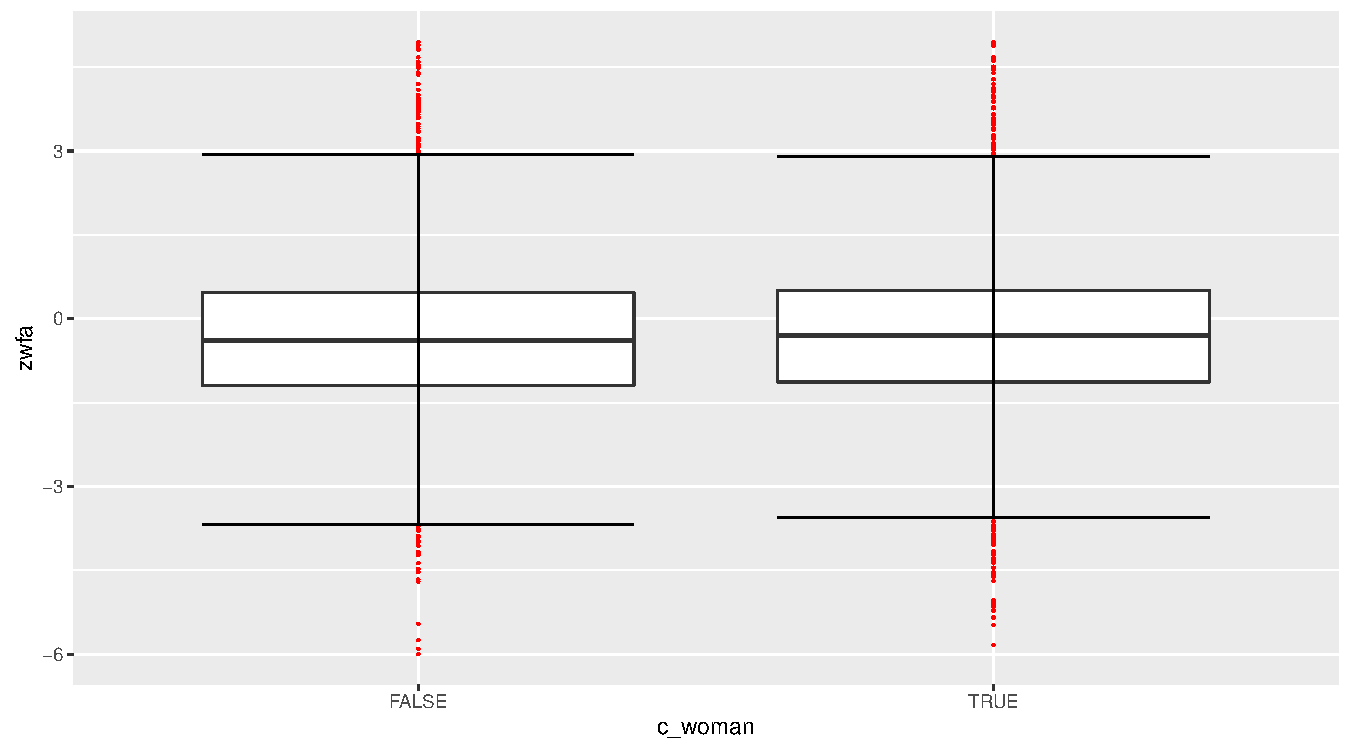
\includegraphics[width=\maxwidth]{figures/latex-waz_boxplot-1} 

\end{knitrout}
\end{figure}

\begin{figure}[H]
\begin{centering}
\caption{Height-for-Age z-score distributions}
\label{tab:haz_descr}
\par\end{centering}
\begin{knitrout}
\definecolor{shadecolor}{rgb}{0.969, 0.969, 0.969}\color{fgcolor}
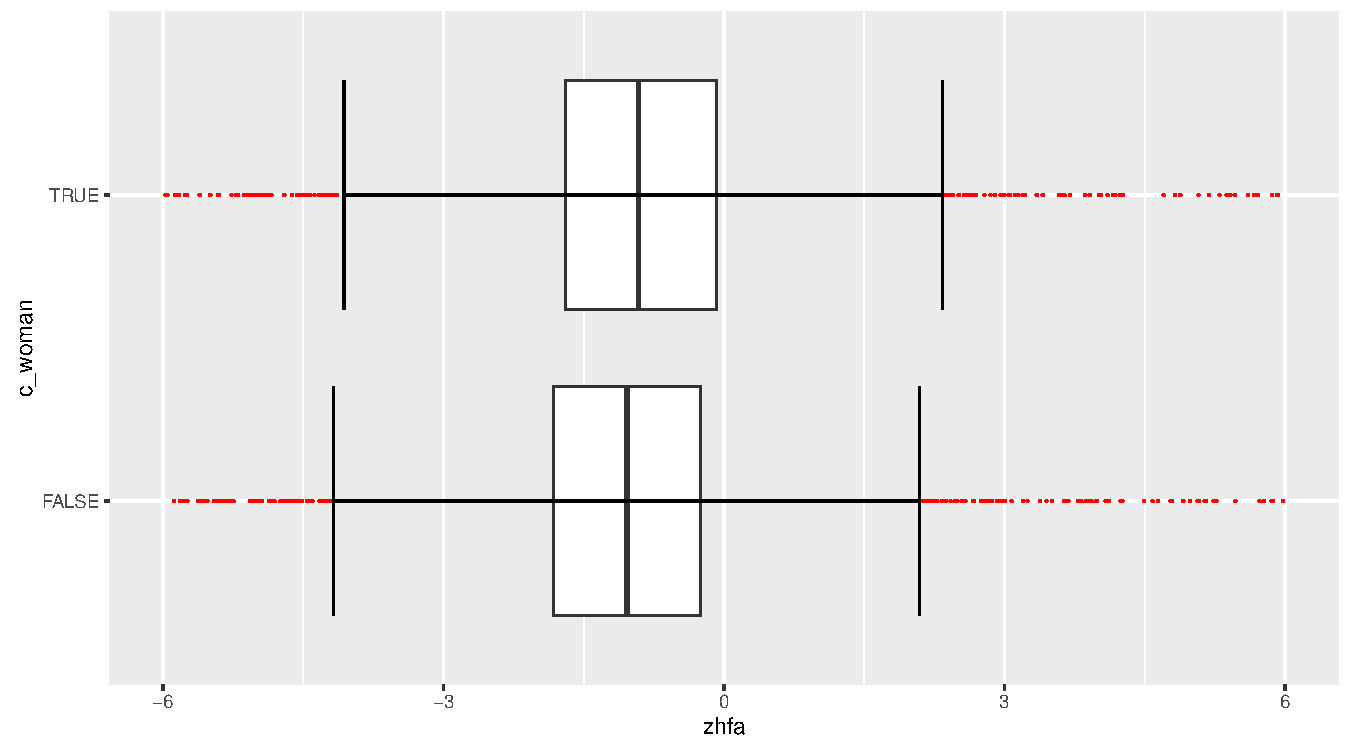
\includegraphics[width=\maxwidth]{figures/latex-haz_boxplot-1} 

\end{knitrout}
\end{figure}

\begin{table}[bh]
\begin{centering}
\caption{Food expenditure }
\label{tab:expf_descr}
\par\end{centering}
\begin{knitrout}
\definecolor{shadecolor}{rgb}{0.969, 0.969, 0.969}\color{fgcolor}


\begin{tabular}{r|r|r|r|r|r|r|r}
\hline
wave & minimum & q1 & median & mean & q3 & maximum & NA's\\
\hline
1 & 24 & 500 & 730 & 947 & 1148 & 14780 & NA\\
\hline
2 & 33 & 560 & 841 & 1015 & 1219 & 27380 & 1456\\
\hline
3 & 30 & 600 & 820 & 1061 & 1216 & 30000 & 944\\
\hline
\end{tabular}
\end{knitrout}
\end{table}

Income from the state pension system is generally the same at slightly
more than 1000 ZAR, which is about half of median income in the data
set.

I construct a dummy variable for children living in a household with
a man aged 60 until 65 (\code{man\_60\_65}). As well as dummies for
a man 65 years or older (\code{man\_65}) and these same dummies for
children living with women of those ages. The interaction of this
dummy variable with the event dummy \code{post\_treatment} is the
variable of interest.

In addition to the explanandum, a number of relevant covariates are
included on the RHS. \tabref{income} gives a description of the distribution
of income as found in the NIDS dataset.

\begin{table}[hb!]
\begin{centering}
\caption{Income distribution}
\label{tab:income}
\par\end{centering}
\begin{knitrout}
\definecolor{shadecolor}{rgb}{0.969, 0.969, 0.969}\color{fgcolor}


\begin{tabular}{r|r|r|r|r|r|r|r}
\hline
wave & minimum & q1 & median & mean & q3 & maximum & NA's\\
\hline
1 & 0.0 & 1284 & 2165 & 4014 & 3966 & 130000 & NA\\
\hline
2 & 100.0 & 1500 & 2583 & 4720 & 4817 & 446900 & 1089\\
\hline
3 & 126.2 & 1980 & 3376 & 5541 & 5933 & 300200 & 944\\
\hline
\end{tabular}
\end{knitrout}
\end{table}

In 2006 the WHO published its standards for child growth\citep{who2006child},
superseding the previously used CDC Growth Charts of \citep[CDC Growth Charts: United States]{nchs2000cdc}.
The WHO charts map the average growth of an ethnically varied sample
of children living in households with healthy lifestyles, setting
a benchmark for growth.

These z-score anthropometrics are used since they are considered to
be a good representation of a child's health. 

For instance, if we measure a height $x$ for a child of age $y$
(in weeks/months), then we refer the to WHO tables, find the relevant
ideal height and standard deviation for a child of age $y$. We then
subtract the ideal height ($\mu_{y}$) from the observed height, and
divide by the standard deviation ($\sigma_{y}$), like so: 
\[
z_{xy}=\frac{x-\mu_{y}}{\sigma_{y}}
\]
These ideal scores are based on a sample of children from different
ethnic populations, in households which observed a healthy lifestyle.
Any health issues, such as malnutrition or disease will affect these
metrics, by causing the child to be shorter or lighter as compared
to these ideal standards. It is however not possible to distinguish
between the different causes of an observed slowed growth.

It is best practice to use only metrics for children between the ages
of 6 months and 60 months.

Here we use two type of z-scores, the Height-for-Age Z-score (HAZ)
and the Weight-for-Age Z-score (WAZ). Since these metrics are both
age-based, they provide information about all past growth issues.
Any past issues such a malnutrition and disease will have impaired
growth, and these effects will still be captured by today's height.
This also applies to the WAZ, as the ideal weight is a function of
the height, which is in turn a function of the age.

These are constructed on a weekly basis up to the age of 60 months,
and on a monthly basis thereafter.

The NIDS uses a file and data structure which is ill suited for panel
data analysis. I therefore transform the data to a format which is
more conducive to panel data analysis. For this I used `Tidy Data'
structure, as described in \citet{wickham2014tidy}.

\section{Empirical methodology}

\label{sec:methodology} The identification strategy in this paper
is based on a policy change in the pension eligibility age for men.
Until the middle of 2009, men became eligible for the state pension
at the age of 65. Between mid 2009 and December 31st 2010, this was
gradually lowered to 60. I combine this information with data from
the South-African National Income Dynamics Study, a full-panel dataset,
which contains information on households from before and after this
policy change. This policy change falls between waves 1 and 2 of the
NIDS, which took place in 2008 and 2011 respectively.

I study the effect of this policy change, on the anthropometric status
of children in the same household as pension recipients as well as
on food and non-food expenditure. 

This identification strategy is operationalised by constructing a
policy change or event dummy. This event dummy is called \code{event},
and takes the value \code{1} for data after the policy change (waves
2 \& 3), and the value \code{0} before the policy change (wave 1).
This dummy is interacted with a dummy variable on having a male household
member aged between 60 and 65 (\code{man\_60\_65}), as well as with
dummies for men age 65 or older and dummies for women of the same
ages.

In order to identify the effect of the policy change, I employ Difference-in-Differences,
using the fixed-effects estimator (the Hausman test rejected random
effects as biased, see \secref{add_estimates}). Based on this setup,
I formulate two base models. One model with the \code{event} dummy,
and an interaction term with male pension recipient (\code{man\_60\_65}).
The second model has the \code{event} dummy and an interaction term
with the same \code{man\_60\_65} dummy, as well as interaction terms
with the dummies for women between 60 and 65 and women and men 65
and above. Each of these models is estimated with both types of z-scores,
as well as food and non-food expenditure as dependent variables.

The outcome variable is $y_{it}$, this outcome variable takes the
form of the of the z-scores, such as HAZ or WAZ or food/non-food expenditure.
Here $t$ denotes time and $i$ the individual. The individual and
time fixes effects are denoted by $\gamma_{i}$ and $\lambda_{t}$
respectively. Dummies for living in a household with a female or a
male pension recipient are included as $P_{it}^{f}$ and $P_{it}^{m}$
respectively. The dummy variable $T_{it}$ denoted the treatment status.
Lastly, $\epsilon_{it}$ is the error term, which is assumed to be
distributed as $\epsilon_{it}\sim N(0,\sigma)$.

\begin{equation}
y_{it}=\alpha_{i}+\lambda_{t}+\delta D{}_{it}+\beta X_{it}+\epsilon_{it}\label{eq:m1}
\end{equation}

In this, $\alpha_{i}$ represents the individual fixed effects, $\lambda_{t}$
represent the time fixed effects, and $X_{it}$ are the time varying
covariates. The error term is $\epsilon_{it}$. Finally the term of
interest is $D_{it}$ . 

The event variable \code{event} is a dummy which takes the value
\code{TRUE} (i.e. \code{1}) for the data collected after the policy
change, i.e. waves 2 and 3 and \code{FALSE} (i.e. \code{0}) for
data collected before then. Lastly, I include the covariate \code{hhincome}
which represents total household income.

As the variables of interest living with a man between 60 and 65,
as well as the other household member dummy variables are determined
at a household level, I apply strandard error corrections to take
this into account, the full procedure is outlined in \secref{add_estimates}.

As described above, I use a total of four dependent variables, Height-for-Age
(HAZ), Weight-for-Age (WAZ), and food and non-food expenditure. Each
of these is used in a different estimation as the Left-Hand Side (LHS)
variable. Combining these four LHSs with each of the three RHSs, gives
a total of twelve estimation equations. I present the results of the
estimation in \secref{results}.

\section{Results}

\label{sec:results} In \tabref{foodexp} I present the result of
the estimations with food and non-food expenditure as dependent variables.
In \tabref{WAZ-full} and \tabref{HAZ-full} I present the estimation
results for the equations with anthropometric status as the dependent
variables. The first four items in each table represent the interaction
terms between the event dummy and the various household member dummies,
e.g. the variable \code{man\_60\_65} is a dummy variable for the
child living in the same household as a male aged 60 until 65.

The other rows represent the independent variables. Where \code{woman\_60\_65}
represents the dummy variable for children living in a household with
a state pension eligible woman aged 60 until 65. The variables \code{man\_65}
and \code{woman\_65} represent pension eligible men an women over
the age of 65 respectively. 

As mentioned in \secref{methodology} I estimate the equations using
only the interaction term with man\_60\_65 as well as with all household
member of age dummies, such as woman\_65, etc. I only present the
results here using all interaction terms. The estimates with the sole
interaction term are qualitatively and quantitatively similar to the
full estimates and are available in \secref{add_estimates}.

\begin{table}[H]

\caption{Food and Non-Food Expenditure}

\begin{centering}
\label{tab:foodexp}
\par\end{centering}
\centering{}%
\begin{tabular}{l|rl|rl}
\hline 
 &
Food &
(P > |t|) &
Non-Food &
(P > |t|)\tabularnewline
\hline 
event {*} Man 60-65 &
\textbf{103.82} &
(0.03) &
-0.05 &
(0.22)\tabularnewline
event {*} Man 65+ &
0.09 &
(1.00) &
-0.02 &
(0.35)\tabularnewline
event {*} Woman 60-65 &
4.69 &
(0.90) &
0.02 &
(0.36)\tabularnewline
event {*} Woman 65+ &
\textbf{104.24} &
(0.00) &
0.01 &
(0.51)\tabularnewline
Man 60-65 &
55.61 &
(0.20) &
206.16 &
(0.57)\tabularnewline
Man 65+ &
\textbf{112.18} &
(0.00) &
377.43 &
(0.57)\tabularnewline
Woman 60-65 &
46.88 &
(0.13) &
-356.02 &
(0.16)\tabularnewline
Woman 65+ &
\textbf{-0.68} &
(0.00) &
-181.57 &
(0.38)\tabularnewline
event &
35.23 &
(0.00) &
131.32 &
(0.08)\tabularnewline
Household Income &
\textbf{0.03} &
(0.00) &
\textbf{0.09} &
(0.00)\tabularnewline
Girl &
-12.49 &
(0.22) &
 &
\tabularnewline
Intercept &
\textbf{810.81} &
(0.00) &
 &
\tabularnewline
\hline 
Observations &
15938 &
 &
15938 &
\tabularnewline
\end{tabular}
\end{table}

The key result in \ref{tab:foodexp} is the coefficient estimate for
the interaction term event {*} man\_60\_65, which is positive at 103.82
with a corresponding p-value of 0.03. This coefficient estimate represents
a 103.82 Rand (ZAR) increase on food expenditure in the households
which received the additional income through pension receipts of men
aged between 60 and 65.

The coefficient estimates for the other independent variables expected
forms. The estimate for household income is positive at 0.03 and highly
significant at 0.00. 

\begin{table}[H]
\caption{Weight for Age}

\begin{centering}
\label{tab:WAZ-full}
\par\end{centering}
\centering{}%
\begin{tabular}{l|lrl|rl|rl}
\hline 
 &
 &
General &
(P > |t|) &
Boys &
(P > |t|) &
Girls &
(P > |t|)\tabularnewline
\hline 
event {*} Man 60-65 &
 &
\textbf{0.33} &
(0.02) &
\textbf{0.44} &
(0.03) &
0.26 &
(0.23)\tabularnewline
event {*} Man 65+ &
 &
-0.03 &
(0.74) &
0.15 &
(0.31) &
\textbf{-0.30} &
(0.05)\tabularnewline
event {*} Woman 60-65 &
 &
0.15 &
(0.18) &
0.18 &
(0.23) &
0.13 &
(0.44)\tabularnewline
event {*} Woman 65+ &
 &
0.04 &
(0.58) &
0.29 &
(0.79) &
0.03 &
(0.77)\tabularnewline
Man 60-65 &
 &
\textbf{-0.27} &
(0.03) &
\textbf{-0.35} &
(0.06) &
-0.29 &
(0.13)\tabularnewline
Man 65+ &
 &
-0.06 &
(0.47) &
\textbf{-0.35} &
(0.01) &
\textbf{0.26} &
(0.04)\tabularnewline
Woman 60-65 &
 &
\textbf{-0.17} &
(0.06) &
-0.14 &
(0.27) &
-0.18 &
(0.21)\tabularnewline
Woman 65+ &
 &
0.03 &
(0.69) &
0.09 &
(0.32) &
-0.02 &
(0.80)\tabularnewline
event &
 &
\textbf{0.00} &
(0.00) &
0.01 &
(0.85) &
0.06 &
(0.19)\tabularnewline
Household Income &
 &
\textbf{0.00} &
(0.00) &
\textbf{0.00} &
(0.00) &
0.00 &
(0.00)\tabularnewline
Girl &
 &
\textbf{0.09} &
(0.00) &
 &
 &
 &
\tabularnewline
Intercept &
 &
\textbf{-0.31} &
(0.00) &
\textbf{-0.33} &
(0.00) &
\textbf{-0.23} &
(0.00)\tabularnewline
\hline 
Observations &
 &
11740 &
 &
5878 &
 &
5862 &
\tabularnewline
\end{tabular}
\end{table}

When using Weight-for-Age as a dependent variable, the coefficient
of interest is positive at 0.33 and significant, with a p-value of
0.02. This respresents an increase of 33\% of a standard deviation
of the WHO Child Growth Standards towards the WHO target mean value.

The interaction terms of the event dummy with the other household
member dummies, \code{man\_65}, \code{woman\_60\_65}, and \code{woman\_65},
are not significant with p-values of 0.74, 0.18, and 0.58 respectively.
A graphical illustration of this result can be seen in \figref{waz-bars},
which shows the average lag in \code{zwfa} for children living with
a man between 60 and 65, before and after the policy change on the
left, as compared to children who do not have such a household member
on the right. 

I also estimate this equation separately for boys and for girls. The
estimation including only boys gives a somewhat higher estimate of
0.44, with a p-value of 0.03. The estimate for girls is lower at 0.26
and insignificant at a p-value of 0.23.

\begin{figure}[H]
\caption{Weight for Age}

\label{fig:waz-bars}

\begin{knitrout}
\definecolor{shadecolor}{rgb}{0.969, 0.969, 0.969}\color{fgcolor}
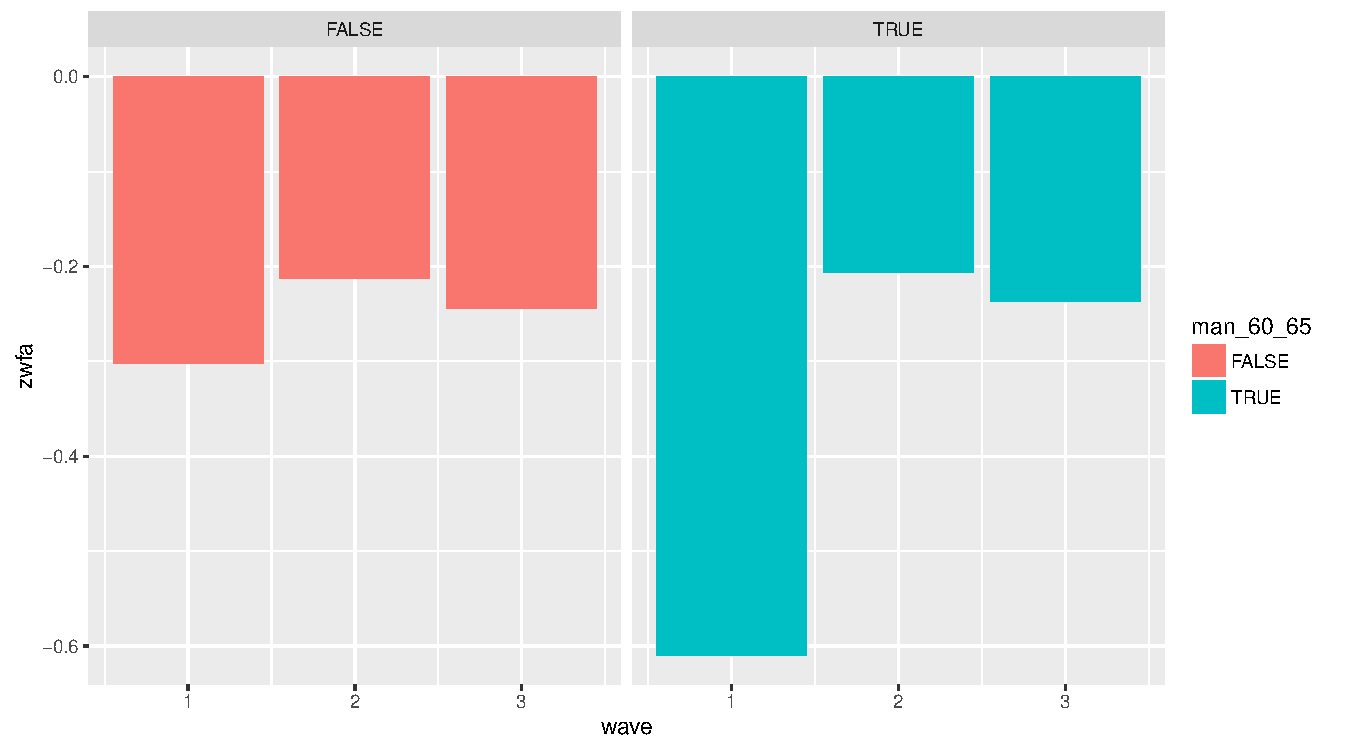
\includegraphics[width=\maxwidth]{figures/latex-waz1-1} 

\end{knitrout}
\end{figure}

When I use Height-for-Age as a dependent variable to result found
is the opposite. I find a negative effect -0.52 of the treatment on
the dependent variable, at a p-value of 0.09. This represents a drop
of 52\% of a standard deviation in the WHO Child Growth Standards,
falling futher below the WHO target mean value.

None of the interaction terms with any of the other household member
dummies are significant, at p-values of 0.31, 0.24, and 0.98 respectively.
When I reestimate the equation to only include boys in the sample,
I find a much greater effect of -0.94, which is also more significant,
at a p-value of 0.04. The same is not true of the restimation which
only includes girls, where the estimate is -0.24 and entirely insignificant
at a p-value of 0.57.

The coefficient estimate for Girl is 0.09, which means that on average
across all three waves, girls z-scores are 9\% of a WHO standard deviation
less below the WHO target mean value than boys are.

The value of the household income coefficient is very low (rounded
to 0.00) but highly significant at a p-value of 0.00, this is simply
because the margin effect of one additional Rand is very small but
nevertheless decisively positive.

\begin{table}[H]
\caption{Height for Age}

\begin{centering}
\label{tab:HAZ-full}
\par\end{centering}
\centering{}%
\begin{tabular}{l|ll|ll|ll}
\hline 
 &
General &
(P > |t|) &
Boys &
(P > |t|) &
Girls &
(P > |t|)\tabularnewline
\hline 
event {*} Man 60-65 &
\textbf{-0.52} &
(0.09) &
\textbf{-0.94} &
\multirow{1}{*}{(0.04)} &
-0.24 &
(0.57)\tabularnewline
event {*} Man 65+ &
-0.23 &
(0.31) &
-0.03 &
(0.92) &
-0.36 &
(0.25)\tabularnewline
event {*} Woman 60-65 &
0.27 &
(0.24) &
0.55 &
(0.08) &
0.02 &
(0.95)\tabularnewline
event {*} Woman 65+ &
-0.00 &
(0.98) &
-0.16 &
(0.49) &
0.14 &
(0.54)\tabularnewline
Man 60-65 &
0.11 &
(0.66) &
0.35 &
0.37 &
-0.06 &
(0.85)\tabularnewline
Man 65+ &
0.19 &
(0.29) &
-0.07 &
(0.79) &
0.42 &
(0.08)\tabularnewline
Woman 60-65 &
\textbf{-0.32} &
(0.08) &
-0.26 &
(0.32) &
-0.40 &
(0.15)\tabularnewline
Woman 65+ &
0.04 &
(0.74) &
0.12 &
(0.50) &
-0.03 &
(0.88)\tabularnewline
event &
-0.01 &
(0.867) &
0.01 &
(0.92) &
-0.03 &
(0.77)\tabularnewline
Household Income &
\textbf{0.00} &
(0.00) &
0.00 &
(0.00) &
\textbf{0.00} &
(0.00)\tabularnewline
Girl &
\textbf{0.22} &
(0.00) &
 &
 &
 &
\tabularnewline
Intercept &
\textbf{-1.30} &
(0.00) &
\textbf{-1.30} &
(0.00) &
\textbf{-1.08} &
(0.00)\tabularnewline
\hline 
Observations &
4809 &
 &
2301 &
 &
2377 &
\tabularnewline
\end{tabular}
\end{table}


\section{Conclusions and limitations}

\label{sec:conclusions}The impetus for this paper is to gain a greater
understanding of the efficiency of cash transfers to male household
members, to for instance improve the designs of CCTs.

I analyse data from the National Income Dynamics Study around a lowering
of the pension eligibility age for men, from 65 to 60, in the South
African state pension system.

Using a Difference-in-Differences based identification strategy, I
compare differences in the anthropometric status of children living
in the same household as men of the newly eligible age.

On the Right-Hand Side I use a dummy variable for the policy change
as well as dummy variables for men aged 60-65, men age 65+ and the
same ones for women as household members. On the Left-Hand Side (LHS)
I use two different anthropometric z-scores, Height-for-Age (HAZ)
and Weight-for-Age as well as food en non-food expenditure. In addition
to the general estimates using z-scores as a dependent variable, I
also reestimate these two equations once using only boys in sample
and once using only girls.

The estimation of these equations gives three key results. Firstly,
I find that there is a significant and consistent positive effect
of the interaction term of the event dummy and the man\_60\_65 dummy,
on food expenditure. Secondly, there is a significant and consistent
positive effect of the same interaction term on the Weight-for-Age
Z-score, the interaction terms with other household member dummies
are not significant. Thirdly, I find a consistent and negative effect
of the interaction term on the Height-for-Age Z-scores. All of these
effect are consistent across the different specifications as well
as standard error corrections.

These effects suggest that the male income resulted in greater food
expenditure, which improved the Weight-for-Height anthropometric status.
Since the estimation includes data from two waves after the policy
change, we would expect this additional food expenditure to also lead
to an improvement in the more long-term metric of Height-for-Age.
Surprisingly we observe an opposite effect here. An explation for
this could be that nature of the expenditure on food has changed,
helping improve the Weight-for-Age, but not improving the Height-for-Age,
with the later being a more long term health indicator.

When I subset to a data to only includes girls and reestimate the
equation with the two z-score dependent variables, I find no significant
effects. However, using a subset of only boys gives the same results
as in the original estimation and at greater significance levels.
This makes it unlikely that the surprising deterioration in Height-for-Age
can be attributed to another factor such as the 2008 global financial
crisis, since this would in all likelyhood also have affected girls
as it did boys.

More central to this study, it suggest that the cash transfer only
affected boys living with a new recipient. As shown in \tabref{waz_descr},
the boys in the dataset scored slightly worse in the Weight-for-Height
z-scores. One possible explanation for the improvement in Weight-for-Age
in boys could be that they benefitted more in terms of this metric
because they were behind more. However, this is at odds with the detioration
in Height-for-Age, since also here, boys scored worse even in wave
1 of the dataset. Should a greater lag have been the cause of the
effect in the improvement in Weight-for-Height then we would expect
a similar improvement in Height-for-Age.

An alternative explanation could be that if the cash transfer was
used to purchase unhealthy food, which increases weight but is not
nutritious in terms of promoting growth, than this was only spent
on boys in the household. If there is merit to this last explanation,
then this result mirrors the result found in \citet{duflo2000child,duflo2003grandmothers},
where the central result is an improvement in girls anthropometric
status when they live with a female pension recipient.

The first key outcome of this research is that food expenditure is
some way too ambiguous a variable. The results of the increased food
expenditure are not altogether positive, leading to a deterioration
in Height-for-Age. In context such as these, the increased food expenditure
would generally be thought of as a positive development. By further
analysing the types of food purchased, it might be possible to better
understand the deterioration in Height-for-Age.

The second key outcome of this research is that both the positive
and negative consequence of the male-only cash transfer seem to only
effect boys. This could suggest that, similarly to \citet{duflo2000child,duflo2003grandmothers}
the grandparent seems to spend only on grandchildren of the same sex.

\printbibliography

%\begin{subappendices}\newpage{}

\appendix

\section{Additional Estimates}

\label{sec:add_estimates}

\begin{table}[H]
\caption{Standard Error Correction}

\begin{knitrout}
\definecolor{shadecolor}{rgb}{0.969, 0.969, 0.969}\color{fgcolor}\begin{kframe}
\begin{alltt}
\hlkwd{library}\hlstd{(lmtest)}  \hlcom{# standard error correction}
\hlkwd{library}\hlstd{(broom)}   \hlcom{# output formatting}

\hlcom{# standard error correction}
\hlkwd{tidy}\hlstd{(} \hlkwd{coeftest}\hlstd{(expf1,} \hlkwc{vcov}\hlstd{=}\hlkwd{vcovHC}\hlstd{(expf1,}
                                  \hlkwc{type}\hlstd{=}\hlstr{"HC0"}\hlstd{,}
                                  \hlkwc{cluster}\hlstd{=}\hlstr{"group"}\hlstd{)) )}
\end{alltt}
\end{kframe}


\begin{tabular}{l|r|r|r|r}
\hline
term & estimate & std.error & statistic & p.value\\
\hline
(Intercept) & 797.973137 & 20.4834004 & 38.957064 & 0.0000000\\
\hline
post\_treatmentTRUE & 54.598225 & 9.4195865 & 5.796244 & 0.0000000\\
\hline
man\_60\_65TRUE & 60.992207 & 30.8335999 & 1.978109 & 0.0479254\\
\hline
man\_65TRUE & 112.135045 & 19.9611804 & 5.617656 & 0.0000000\\
\hline
woman\_60\_65TRUE & 47.634524 & 15.3353771 & 3.106185 & 0.0018969\\
\hline
woman\_65TRUE & 3.158883 & 12.1322850 & 0.260370 & 0.7945802\\
\hline
hhincome & 0.034387 & 0.0047316 & 7.267585 & 0.0000000\\
\hline
womanTRUE & -12.610512 & 10.1037207 & -1.248106 & 0.2120019\\
\hline
post\_treatmentTRUE:man\_60\_65TRUE & 97.758973 & 39.4529129 & 2.477864 & 0.0132225\\
\hline
\end{tabular}
\end{knitrout}
\end{table}

\begin{table}[H]
\begin{centering}
\caption{Non-food expenditure }
\label{tab:expnf_descr}
\par\end{centering}
\begin{knitrout}
\definecolor{shadecolor}{rgb}{0.969, 0.969, 0.969}\color{fgcolor}\begin{kframe}
\begin{alltt}
\hlstd{NIDS} \hlopt
  \hlkwd{group_by}\hlstd{(wave)} \hlopt
  \hlkwd{do}\hlstd{(}\hlkwd{tidy}\hlstd{(}\hlkwd{summary}\hlstd{(.}\hlopt{$}\hlstd{expnf)))}
\end{alltt}
\end{kframe}


\begin{tabular}{r|r|r|r|r|r|r|r}
\hline
wave & minimum & q1 & median & mean & q3 & maximum & NA's\\
\hline
1 & 4.000 & 220.0 & 552.4 & 1789 & 1425 & 120300 & NA\\
\hline
2 & 1.000 & 285.1 & 588.1 & 1678 & 1300 & 361000 & 1456\\
\hline
3 & 4.429 & 336.0 & 755.0 & 1870 & 1735 & 112000 & 944\\
\hline
\end{tabular}
\end{knitrout}
\end{table}

\begin{table}[H]
\caption{Non-Food Expenditure}

\label{tab:expnf}

\begin{knitrout}
\definecolor{shadecolor}{rgb}{0.969, 0.969, 0.969}\color{fgcolor}\begin{kframe}
\begin{alltt}
\hlkwd{plm}\hlstd{(expnf} \hlopt{~}     \hlstd{post_treatment}\hlopt{*}\hlstd{post_treatment} \hlopt{+}
                \hlstd{man_65} \hlopt{+}
                \hlstd{wopost_treatment} \hlopt{+}
                \hlstd{woman_65} \hlopt{+}
                \hlstd{hhincome} \hlopt{+}
                \hlstd{woman,}
                \hlkwc{data}   \hlstd{= NIDS,}
                \hlkwc{model}  \hlstd{=} \hlstr{'random'}\hlstd{)}
\end{alltt}
\end{kframe}
\end{knitrout}

\begin{knitrout}
\definecolor{shadecolor}{rgb}{0.969, 0.969, 0.969}\color{fgcolor}
\begin{tabular}{l|r|r|r|r}
\hline
  & Estimate & Std. Error & t-value & Pr(>|t|)\\
\hline
(Intercept) & 1052.4112911 & 56.710077 & 18.5577476 & 0.0000000\\
\hline
post\_treatmentTRUE & -229.1189649 & 53.971673 & -4.2451707 & 0.0000219\\
\hline
man\_60\_65TRUE & -12.9406582 & 245.515119 & -0.0527082 & 0.9579648\\
\hline
man\_65TRUE & -345.7800113 & 96.666790 & -3.5770300 & 0.0003481\\
\hline
woman\_60\_65TRUE & -385.0294955 & 93.983693 & -4.0967692 & 0.0000420\\
\hline
woman\_65TRUE & -617.4061057 & 70.636448 & -8.7406166 & 0.0000000\\
\hline
hhincome & 0.2310988 & 0.003067 & 75.3510870 & 0.0000000\\
\hline
womanTRUE & -52.8786218 & 54.028761 & -0.9787125 & 0.3277298\\
\hline
post\_treatmentTRUE:man\_60\_65TRUE & -231.9316003 & 281.149594 & -0.8249402 & 0.4094120\\
\hline
\end{tabular}


\end{knitrout}
\end{table}

\begin{table}[H]
\caption{Food Expenditure Interact All}

\label{tab:expf2}

\begin{knitrout}
\definecolor{shadecolor}{rgb}{0.969, 0.969, 0.969}\color{fgcolor}\begin{kframe}
\begin{alltt}
\hlkwd{plm}\hlstd{(expf} \hlopt{~}      \hlstd{post_treatment}\hlopt{*}\hlstd{post_treatment} \hlopt{+}
                \hlstd{post_treatment}\hlopt{*}\hlstd{man_65} \hlopt{+}
                \hlstd{post_treatment}\hlopt{*}\hlstd{wopost_treatment} \hlopt{+}
                \hlstd{post_treatment}\hlopt{*}\hlstd{woman_65} \hlopt{+}
                \hlstd{hhincome} \hlopt{+}
                \hlstd{woman,}
                \hlkwc{data}   \hlstd{= NIDS,}
                \hlkwc{model}  \hlstd{=} \hlstr{'within'}\hlstd{)}
\end{alltt}
\end{kframe}
\end{knitrout}

\begin{knitrout}
\definecolor{shadecolor}{rgb}{0.969, 0.969, 0.969}\color{fgcolor}
\begin{tabular}{l|r|r|r|r}
\hline
  & Estimate & Std. Error & t-value & Pr(>|t|)\\
\hline
(Intercept) & 810.8105328 & 10.8755576 & 74.5534680 & 0.0000000\\
\hline
post\_treatmentTRUE & 35.2251442 & 10.5897866 & 3.3263318 & 0.0008810\\
\hline
man\_60\_65TRUE & 55.6196875 & 43.0213993 & 1.2928377 & 0.1960770\\
\hline
man\_65TRUE & 112.1835241 & 28.5781790 & 3.9254959 & 0.0000867\\
\hline
woman\_60\_65TRUE & 46.8846693 & 30.9664240 & 1.5140485 & 0.1300239\\
\hline
woman\_65TRUE & -67.8984723 & 21.0318516 & -3.2283640 & 0.0012463\\
\hline
hhincome & 0.0344025 & 0.0005493 & 62.6291630 & 0.0000000\\
\hline
womanTRUE & -12.4862470 & 10.2886736 & -1.2135915 & 0.2249131\\
\hline
post\_treatmentTRUE:man\_60\_65TRUE & 103.8232181 & 49.1094384 & 2.1141194 & 0.0345132\\
\hline
post\_treatmentTRUE:man\_65TRUE & 0.0905759 & 33.1925710 & 0.0027288 & 0.9978228\\
\hline
post\_treatmentTRUE:woman\_60\_65TRUE & 4.6874243 & 35.5632106 & 0.1318054 & 0.8951391\\
\hline
post\_treatmentTRUE:woman\_65TRUE & 104.2408234 & 24.1584808 & 4.3148749 & 0.0000160\\
\hline
\end{tabular}


\end{knitrout}
\end{table}

\begin{table}[H]
\caption{Girls Height for Age}

\begin{knitrout}
\definecolor{shadecolor}{rgb}{0.969, 0.969, 0.969}\color{fgcolor}\begin{kframe}
\begin{alltt}
\hlkwd{plm}\hlstd{(zhfa} \hlopt{~}      \hlstd{post_treatment}\hlopt{*}\hlstd{man_60_65} \hlopt{+}
                \hlstd{post_treatment}\hlopt{*}\hlstd{man_65} \hlopt{+}
                \hlstd{post_treatment}\hlopt{*}\hlstd{woman_60_65} \hlopt{+}
                \hlstd{post_treatment}\hlopt{*}\hlstd{woman_65} \hlopt{+}
                \hlstd{hhincome,}
                \hlkwc{data} \hlstd{= NIDS,}
                \hlkwc{subset} \hlstd{= best_age_yrs} \hlopt{<} \hlnum{4} \hlopt{&}
                \hlstd{woman} \hlopt{==} \hlnum{TRUE}\hlstd{,}
                \hlkwc{model}\hlstd{=}\hlstr{'between'}\hlstd{)}
\end{alltt}
\end{kframe}
\end{knitrout}

\begin{knitrout}
\definecolor{shadecolor}{rgb}{0.969, 0.969, 0.969}\color{fgcolor}
\begin{tabular}{l|r|r|r|r}
\hline
  & Estimate & Std. Error & t-value & Pr(>|t|)\\
\hline
(Intercept) & -1.0827829 & 0.0853476 & -12.6867426 & 0.0000000\\
\hline
eventTRUE & -0.0292989 & 0.1014385 & -0.2888346 & 0.7727352\\
\hline
man\_60\_65TRUE & -0.0656365 & 0.3501531 & -0.1874508 & 0.8513245\\
\hline
man\_65TRUE & 0.4217243 & 0.2468947 & 1.7081136 & 0.0877565\\
\hline
woman\_60\_65TRUE & -0.3987542 & 0.2798468 & -1.4249014 & 0.1543277\\
\hline
woman\_65TRUE & -0.0273289 & 0.1885614 & -0.1449338 & 0.8847765\\
\hline
hhincome & 0.0000250 & 0.0000058 & 4.3324668 & 0.0000154\\
\hline
eventTRUE:man\_60\_65TRUE & -0.2353016 & 0.4120205 & -0.5710920 & 0.5679957\\
\hline
eventTRUE:man\_65TRUE & -0.3603559 & 0.3146522 & -1.1452513 & 0.2522298\\
\hline
eventTRUE:woman\_60\_65TRUE & 0.0214524 & 0.3339310 & 0.0642420 & 0.9487834\\
\hline
eventTRUE:woman\_65TRUE & 0.1394328 & 0.2329406 & 0.5985769 & 0.5495168\\
\hline
\end{tabular}


\end{knitrout}
\end{table}

\begin{table}[H]
\caption{Boys Height for Age}

\begin{knitrout}
\definecolor{shadecolor}{rgb}{0.969, 0.969, 0.969}\color{fgcolor}\begin{kframe}
\begin{alltt}
\hlkwd{plm}\hlstd{(zhfa} \hlopt{~}      \hlstd{post_treatment}\hlopt{*}\hlstd{man_60_65} \hlopt{+}
                \hlstd{post_treatment}\hlopt{*}\hlstd{man_65} \hlopt{+}
                \hlstd{post_treatment}\hlopt{*}\hlstd{woman_60_65} \hlopt{+}
                \hlstd{post_treatment}\hlopt{*}\hlstd{woman_65} \hlopt{+}
                \hlstd{hhincome,}
                \hlkwc{data} \hlstd{= NIDS,}
                \hlkwc{subset} \hlstd{= best_age_yrs} \hlopt{<} \hlnum{4} \hlopt{&}
                \hlstd{woman} \hlopt{==} \hlnum{FALSE}\hlstd{,}
                \hlkwc{model}\hlstd{=}\hlstr{'between'}\hlstd{)}
\end{alltt}
\end{kframe}
\end{knitrout}

\begin{knitrout}
\definecolor{shadecolor}{rgb}{0.969, 0.969, 0.969}\color{fgcolor}
\begin{tabular}{l|r|r|r|r}
\hline
  & Estimate & Std. Error & t-value & Pr(>|t|)\\
\hline
(Intercept) & -1.2998129 & 0.0848152 & -15.3252272 & 0.0000000\\
\hline
eventTRUE & 0.0103725 & 0.1028205 & 0.1008795 & 0.9196557\\
\hline
man\_60\_65TRUE & 0.3491800 & 0.3913368 & 0.8922751 & 0.3723477\\
\hline
man\_65TRUE & -0.0665181 & 0.2569582 & -0.2588674 & 0.7957629\\
\hline
woman\_60\_65TRUE & -0.2599733 & 0.2609596 & -0.9962203 & 0.3192579\\
\hline
woman\_65TRUE & 0.1223980 & 0.1829573 & 0.6689976 & 0.5035705\\
\hline
hhincome & 0.0000156 & 0.0000065 & 2.3876923 & 0.0170425\\
\hline
eventTRUE:man\_60\_65TRUE & -0.9431906 & 0.4647851 & -2.0293047 & 0.0425532\\
\hline
eventTRUE:man\_65TRUE & -0.0319730 & 0.3231811 & -0.0989320 & 0.9212017\\
\hline
eventTRUE:woman\_60\_65TRUE & 0.5501036 & 0.3207639 & 1.7149798 & 0.0864965\\
\hline
eventTRUE:woman\_65TRUE & -0.1619634 & 0.2326134 & -0.6962771 & 0.4863324\\
\hline
\end{tabular}


\end{knitrout}
\end{table}

\begin{table}[H]
\caption{Height for Age}

\begin{knitrout}
\definecolor{shadecolor}{rgb}{0.969, 0.969, 0.969}\color{fgcolor}\begin{kframe}
\begin{alltt}
\hlkwd{plm}\hlstd{(zhfa} \hlopt{~}      \hlstd{post_treatment}\hlopt{*}\hlstd{man_60_65} \hlopt{+}
                \hlstd{post_treatment}\hlopt{*}\hlstd{man_65} \hlopt{+}
                \hlstd{post_treatment}\hlopt{*}\hlstd{woman_60_65} \hlopt{+}
                \hlstd{post_treatment}\hlopt{*}\hlstd{woman_65} \hlopt{+}
                \hlstd{hhincome} \hlopt{+}
                \hlstd{woman,}
                \hlkwc{data} \hlstd{= NIDS,}
                \hlkwc{subset} \hlstd{= best_age_yrs} \hlopt{<} \hlnum{4}\hlstd{,}
                \hlkwc{model}\hlstd{=}\hlstr{'between'}\hlstd{)}
\end{alltt}
\end{kframe}
\end{knitrout}

\begin{knitrout}
\definecolor{shadecolor}{rgb}{0.969, 0.969, 0.969}\color{fgcolor}
\begin{tabular}{l|r|r|r|r}
\hline
  & Estimate & Std. Error & t-value & Pr(>|t|)\\
\hline
(Intercept) & -1.3045248 & 0.0661855 & -19.7101308 & 0.0000000\\
\hline
post\_treatmentTRUE & -0.0118690 & 0.0722069 & -0.1643745 & 0.8694440\\
\hline
man\_60\_65TRUE & 0.1125166 & 0.2609687 & 0.4311499 & 0.6663809\\
\hline
man\_65TRUE & 0.1873098 & 0.1780119 & 1.0522319 & 0.2927522\\
\hline
woman\_60\_65TRUE & -0.3244063 & 0.1907804 & -1.7004174 & 0.0891246\\
\hline
woman\_65TRUE & 0.0430632 & 0.1312351 & 0.3281375 & 0.7428237\\
\hline
hhincome & 0.0000211 & 0.0000043 & 4.8737618 & 0.0000011\\
\hline
womanTRUE & 0.2245553 & 0.0563309 & 3.9863642 & 0.0000682\\
\hline
post\_treatmentTRUE:man\_60\_65TRUE & -0.5174950 & 0.3081696 & -1.6792542 & 0.0931751\\
\hline
post\_treatmentTRUE:man\_65TRUE & -0.2266029 & 0.2252792 & -1.0058756 & 0.3145319\\
\hline
post\_treatmentTRUE:woman\_60\_65TRUE & 0.2697230 & 0.2306746 & 1.1692789 & 0.2423560\\
\hline
post\_treatmentTRUE:woman\_65TRUE & -0.0021065 & 0.1644171 & -0.0128120 & 0.9897784\\
\hline
\end{tabular}


\end{knitrout}
\end{table}

\begin{table}[H]
\caption{Weight for Age}

\begin{knitrout}
\definecolor{shadecolor}{rgb}{0.969, 0.969, 0.969}\color{fgcolor}\begin{kframe}
\begin{alltt}
\hlkwd{plm}\hlstd{(zwfa} \hlopt{~}      \hlstd{post_treatment}\hlopt{*}\hlstd{man_60_65} \hlopt{+}
                \hlstd{post_treatment}\hlopt{*}\hlstd{man_65} \hlopt{+}
                \hlstd{post_treatment}\hlopt{*}\hlstd{woman_60_65} \hlopt{+}
                \hlstd{post_treatment}\hlopt{*}\hlstd{woman_65} \hlopt{+}
                \hlstd{hhincome} \hlopt{+}
                \hlstd{woman,}
                \hlkwc{data} \hlstd{= NIDS,}
                \hlkwc{subset} \hlstd{= c_age_days1} \hlopt{>} \hlnum{180} \hlopt{&} \hlstd{c_age_days1} \hlopt{<} \hlnum{2920}\hlstd{,}
                \hlkwc{model}\hlstd{=}\hlstr{'between'}\hlstd{)}
\end{alltt}
\end{kframe}
\end{knitrout}

\begin{knitrout}
\definecolor{shadecolor}{rgb}{0.969, 0.969, 0.969}\color{fgcolor}
\begin{tabular}{l|r|r|r|r}
\hline
  & Estimate & Std. Error & t-value & Pr(>|t|)\\
\hline
(Intercept) & -0.3073009 & 0.0326055 & -9.4248055 & 0.0000000\\
\hline
post\_treatmentTRUE & 0.0032539 & 0.0326791 & 0.0995698 & 0.9206876\\
\hline
man\_60\_65TRUE & -0.2768796 & 0.1304236 & -2.1229253 & 0.0337810\\
\hline
man\_65TRUE & -0.0623759 & 0.0854461 & -0.7300029 & 0.4654030\\
\hline
woman\_60\_65TRUE & -0.1747761 & 0.0940851 & -1.8576383 & 0.0632454\\
\hline
woman\_65TRUE & 0.0254201 & 0.0639132 & 0.3977282 & 0.6908378\\
\hline
hhincome & 0.0000100 & 0.0000016 & 6.2361148 & 0.0000000\\
\hline
womanTRUE & 0.0953099 & 0.0293109 & 3.2516874 & 0.0011505\\
\hline
post\_treatmentTRUE:man\_60\_65TRUE & 0.3300113 & 0.1479880 & 2.2299866 & 0.0257672\\
\hline
post\_treatmentTRUE:man\_65TRUE & -0.0333463 & 0.1008261 & -0.3307311 & 0.7408535\\
\hline
post\_treatmentTRUE:woman\_60\_65TRUE & 0.1452480 & 0.1078110 & 1.3472466 & 0.1779269\\
\hline
post\_treatmentTRUE:woman\_65TRUE & 0.0412345 & 0.0738919 & 0.5580384 & 0.5768288\\
\hline
\end{tabular}


\end{knitrout}
\end{table}

\begin{table}[H]
\caption{Food Expenditure}

\begin{centering}
\label{tab:expf}
\par\end{centering}
\begin{knitrout}
\definecolor{shadecolor}{rgb}{0.969, 0.969, 0.969}\color{fgcolor}\begin{kframe}
\begin{alltt}
\hlkwd{plm}\hlstd{(expf} \hlopt{~}      \hlstd{post_treatment}\hlopt{*}\hlstd{man_60_65} \hlopt{+}
                \hlstd{post_treatment}\hlopt{*}\hlstd{man_65} \hlopt{+}
                \hlstd{post_treatment}\hlopt{*}\hlstd{woman_60_65} \hlopt{+}
                \hlstd{post_treatment}\hlopt{*}\hlstd{woman_65} \hlopt{+}
                \hlstd{hhincome} \hlopt{+}
                \hlstd{woman,}
                \hlkwc{data}   \hlstd{= NIDS,}
                \hlkwc{model}  \hlstd{=} \hlstr{'within'}\hlstd{)}
\end{alltt}
\end{kframe}
\end{knitrout}

\begin{knitrout}
\definecolor{shadecolor}{rgb}{0.969, 0.969, 0.969}\color{fgcolor}
\begin{tabular}{l|r|r|r|r}
\hline
  & Estimate & Std. Error & t-value & Pr(>|t|)\\
\hline
(Intercept) & 810.8105328 & 10.8755576 & 74.5534680 & 0.0000000\\
\hline
post\_treatmentTRUE & 35.2251442 & 10.5897866 & 3.3263318 & 0.0008810\\
\hline
man\_60\_65TRUE & 55.6196875 & 43.0213993 & 1.2928377 & 0.1960770\\
\hline
man\_65TRUE & 112.1835241 & 28.5781790 & 3.9254959 & 0.0000867\\
\hline
woman\_60\_65TRUE & 46.8846693 & 30.9664240 & 1.5140485 & 0.1300239\\
\hline
woman\_65TRUE & -67.8984723 & 21.0318516 & -3.2283640 & 0.0012463\\
\hline
hhincome & 0.0344025 & 0.0005493 & 62.6291630 & 0.0000000\\
\hline
womanTRUE & -12.4862470 & 10.2886736 & -1.2135915 & 0.2249131\\
\hline
post\_treatmentTRUE:man\_60\_65TRUE & 103.8232181 & 49.1094384 & 2.1141194 & 0.0345132\\
\hline
post\_treatmentTRUE:man\_65TRUE & 0.0905759 & 33.1925710 & 0.0027288 & 0.9978228\\
\hline
post\_treatmentTRUE:woman\_60\_65TRUE & 4.6874243 & 35.5632106 & 0.1318054 & 0.8951391\\
\hline
post\_treatmentTRUE:woman\_65TRUE & 104.2408234 & 24.1584808 & 4.3148749 & 0.0000160\\
\hline
\end{tabular}


\end{knitrout}
\end{table}

\begin{table}[H]
\caption{Hausmann}

\begin{knitrout}
\definecolor{shadecolor}{rgb}{0.969, 0.969, 0.969}\color{fgcolor}\begin{kframe}
\begin{alltt}
\hlstd{model_expf2} \hlkwb{<-} \hlstd{expnf} \hlopt{~} \hlstd{post_treatment}\hlopt{*}\hlstd{man_60_65} \hlopt{+}
\hlstd{post_treatment}\hlopt{*}\hlstd{man_65} \hlopt{+}
\hlstd{woman_60_65}\hlopt{*}\hlstd{post_treatment} \hlopt{+}
\hlstd{post_treatment}\hlopt{*}\hlstd{woman_65} \hlopt{+}
\hlstd{hhincome} \hlopt{+}
\hlstd{woman}

\hlstd{fe_expf2} \hlkwb{<-} \hlkwd{plm}\hlstd{(model_expf2,} \hlkwc{data}\hlstd{=NIDS,} \hlkwc{model}\hlstd{=}\hlstr{'within'}\hlstd{)}
\end{alltt}
\begin{verbatim}
## series fwag, cwag, swag, chld, fost, spen_flg, ppen_flg, uif, remt are NA and have been removed
## series spen, ppen are constants and have been removed
\end{verbatim}
\begin{alltt}
\hlstd{re_expf2} \hlkwb{<-} \hlkwd{plm}\hlstd{(model_expf2,} \hlkwc{data}\hlstd{=NIDS,} \hlkwc{model}\hlstd{=}\hlstr{'random'}\hlstd{)}
\end{alltt}
\begin{verbatim}
## series fwag, cwag, swag, chld, fost, spen_flg, ppen_flg, uif, remt are NA and have been removed
## series spen, ppen are constants and have been removed
\end{verbatim}
\begin{alltt}
\hlkwd{phtest}\hlstd{(fe_expf2, re_expf2)}
\end{alltt}
\begin{verbatim}
## 
## 	Hausman Test
## 
## data:  model_expf2
## chisq = 857.92, df = 10, p-value < 2.2e-16
## alternative hypothesis: one model is inconsistent
\end{verbatim}
\end{kframe}
\end{knitrout}

\end{table}


\section{Software}

\label{sec:software}The computation estimation of these models is
performed using R \citep{R}, with the implementation of the panel
data structure and models using the \code{plm} package by \citet{croissant2008panel}.
Generalized Linear Models for the panel data set are estimated using
the pglm package by \citet{croissant2013pglm}.

All changes are logged using the version control system Git \citep{git}
and publicly available on GitHub at \href{https://github.com/bquast/MaleFemale-Bargaining-Power-Child-Growth/}{https://github.com/bquast/MaleFemale-Bargaining-Power-Child-Growth/}\footnote{The repository can by cloned to a local computer by entering in following
command in a terminal (with Git installed):\\
\code{git clone https://github.com/bquast/MaleFemale-Bargaining-Power-Child-Growth.git}}.

In order to merge data and compute of these statistics, I make use
of the dplyr and tidyr R packages \citet{wickham2015dplyr,wickham2016tidyr}.
After having combined the various data.frames within each wave, the
three waves can be combined by simply joining the rows using base
R's \code{rbind()} function\citep{R}.

%\end{subappendices}
\end{document}
